%In the current context, dominated by the advent of the Industry 4.0, production systems are characterized by a higher complexity of decision-making processes that are loosely distributed among the CPSs operating along the entire value network. 

FAR-EDGE is a H2020 EU project that has the fundamental goal to devise and develop an integrated Edge Computing platform for the virtualization of the factory automation pyramid that strategically supports  production-related activities during all phases of the engineering and factory life cycle. 
This objective entails the definition and implementation of several software layers serving three high-level functional domains, namely \textit{Automation}, \textit{Analytics}, and \textit{Simulation} (see Figure~\ref{fig:architecture}) to meet the global challenges of mass-customization and reshoring.

\begin{figure}[b]
	\centering
	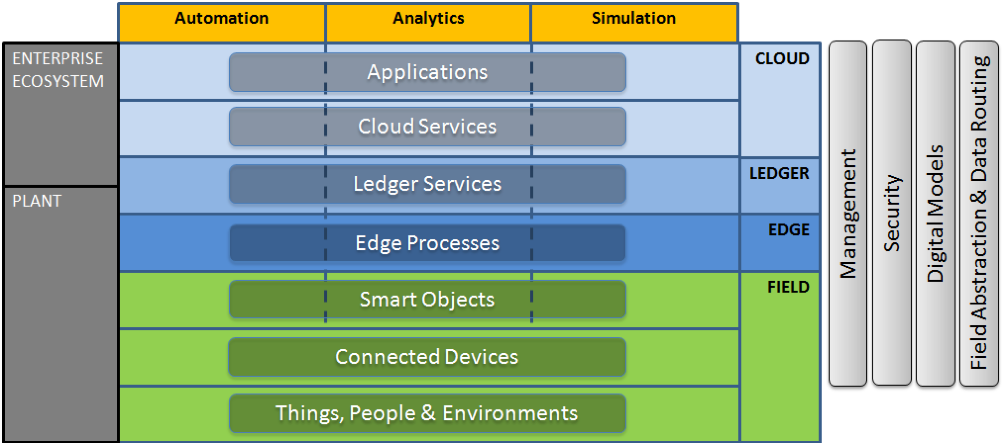
\includegraphics[width=\linewidth]{images/Far-edge.png}
	\caption{FAR-EDGE Reference Architecture overall view}
	\label{fig:architecture}
\end{figure}

As far as simulation is concerned FAR-EDGE aims at providing models and tools encompassing functionalities for modeling CPS-based discrete manufacturing factories and simulating their behavior along the whole factory life cycle. 
FAR-EDGE, in fact, sees simulation as a first-class citizen of the factory of the future (in compliance with the I4.0 guidelines), that is a primary enabler to achieve layout and product optimization, to test \textit{what-if} scenarios at minimal impact of regular shop activities, or as a the cornerstone to make reactive (\textit{now-what}) operative decisions. New simulation services are envisioned which capable to operate near the data sources to support first-time-right solutions to multi-disciplinary issues occurring in production, logistics and management processes.

As it was mentioned in the introduction to this chapter, in the current context, dominated by the advent of the Industry 4.0, production systems are characterized by a higher complexity of decision-making processes that are loosely distributed among the CPSs operating along the entire value network. 
One of the main challenges of applying simulation in manufacturing concerns the pursuit of a continuity between the shop floor and its digital representation that constantly and faithfully reflect the state of the factory throughout its life cycle (\textit{Digital Continuity}).
This need is translated into the definition and put in place of models and techniques to allow the simulation model to be always in sync with the shop floor and automatically evolve with the state of the factory. 
Synchronization and evolution are the two main keywords at this juncture, as CPSs are subject to changes (e.g., for straining and aging), models must reflect those transformations. 
To detect this gap and update the model accordingly FAR-EDGE envisions capturing and exploiting streams of data from the field and processing by analysis algorithms from \textit{Analytics} domain. 
This means that within the simulation domain FAR-EDGE aims at establishing a platform for the real-time collection of data streams originating from the shop floor and their analysis by means of complex algorithms built upon primitives made available by the Analytics domain. 
The system shall be able to automatically and transparently update the model. 
To do this FAR-EDGE proposes a modelling language backed up by an \textit{Open API for Virtualization} based on the concept of CPS that is flexible and open, and natively supports a data transformation to allow a stakeholder to define data analysis processes specific to each CPS.
For all the reasons presented above, the task of defining a suitable platform is ambitious; in fact, not only FAR-EDGE aims at including in a single harmonic, coherent representation control, communication data collection and simulation data, but also at defining and being able to share a model describing the synchronization process. 




